
\de{ĐỀ THI GIỮA HỌC KỲ II NĂM HỌC 2022-2023}{THPT Hàn Thuyên}

\begin{center}
	\textbf{PHẦN 1 - TRẮC NGHIỆM}
\end{center}

\Opensolutionfile{ans}[ans/HanThuyen-GKII-HCM-TNTL]

%Câu 1...........................
\begin{ex}%[0T7Y1-1]%[Dự án đề kiểm tra GKHI NH22-23-Trương Đăng Khoa]%[Trương Đăng Khoa]
Bất phương trình nào sau đây là bất phương trình bậc $2$	một ẩn?
	\choice
	{$2x^3-3x+1\geq 0$}
	{$x^2+y^2\geq 2023$}
	{$x^2-\dfrac{3}{x}<1$}
	{\True $2023x-2024x^2+1<0$}
	\loigiai{
	Bất phương trình trình bậc $2$	một ẩn	là $2023x-2024x^2+1<0$.
	}
\end{ex}

%Câu 2...........................
\begin{ex}%[0T7B2-1]%[Dự án đề kiểm tra GKHI NH22-23-Trương Đăng Khoa]%[Trương Đăng Khoa]
Giải phương trình $\sqrt{3x+13}=x+3$.	
	\choice
	{\True $x=1$}
	{$x=-4$ hoặc $x=1$}
	{$x=-4$}
	{$x=-1$ hoặc $x=4$}
	\loigiai{
	Bình phương hai vế phương trình $\sqrt{3x+13}=x+3$ ta được
	\allowdisplaybreaks
	\begin{eqnarray*}
		&&3x+13=(x+3)^2
		\\
		&\Leftrightarrow&3x+13=x^2+6x+9
		\\
		&\Leftrightarrow&x^2+3x-3=0
		\\
		&\Leftrightarrow&\hoac{&x=1\\&x=-3.}
	\end{eqnarray*}
Thử lại chỉ có $x=1$ thỏa phương trình.\\
Vậy phương trình đã cho có một nghiệm $x=1$.
	}
\end{ex}

%Câu 3...........................
\begin{ex}%[0T7B2-1]%[Dự án đề kiểm tra GKHI NH22-23-Trương Đăng Khoa]%[Trương Đăng Khoa]
Tập nghiệm của bất phương trình $x^2-9\geq 4x(x-3)$	 là 
	\choice
	{\True $[1;3]$}
	{$(1;3)$}
	{$[1;+\infty)$}
	{$(-\infty;1]$}
	\loigiai{
	Ta có 	$x^2-9\geq 4x(x-3)\Leftrightarrow -3x^2+12x-9\geq 0$.\\
	Tam thức $-3x^2+12x-9=0\Leftrightarrow\hoac{&x=1\\&x=3.}$
	\begin{center}
		\begin{tikzpicture}[font=\normalsize,t style/.style={style=solid}]
			\tkzTabInit[nocadre=false,lgt=4,espcl=2.5,deltacl=0.5]
			{$x$ /0.75, $-3x^2+12x-9$/1}
			{$ -\infty $,$ 1 $,$ 3 $,$ +\infty $}
			\tkzTabLine{  , -,0 , +,0  , -,  }  
		\end{tikzpicture}
	\end{center}
	Vậy tập nghiệm của bất phương trình $x^2-9\geq 4x(x-3)$	 là $[1;3]$.
	}
\end{ex}

%Câu 4...........................
\begin{ex}%[0T9Y1-3]%[Dự án đề kiểm tra GKHI NH22-23-Trương Đăng Khoa]%[Trương Đăng Khoa]
Trong mặt phẳng với hệ tọa độ $Oxy$, cho tam giác $ABC$	 có ba đỉnh $A(-1;2)$, $B(2;0)$, $C(-3;1)$. Tọa độ trọng tâm $G$ của tam giác $ABC$ là
	\choice
	{$G\left(\dfrac{2}{3};-1\right)$}
	{$G\left(\dfrac{4}{3};-1\right)$}
	{$G\left(-\dfrac{4}{3};1\right)$}
	{\True $G\left(-\dfrac{2}{3};1\right)$}
	\loigiai{Vì $G$ là trọng tâm của tam giác $ABC$ nên
	ta có $\heva{&x_G=\dfrac{-1+2+(-3)}{3}=-\dfrac{2}{3}\\&y_G=\dfrac{2+0+1}{3}=1.}$	\\
	Vậy $G\left(-\dfrac{2}{3};1\right)$.
	}
\end{ex}

%Câu 5...........................
\begin{ex}%[0T9Y2-1]%[Dự án đề kiểm tra GKHI NH22-23-Trương Đăng Khoa]%[Trương Đăng Khoa]
Véc-tơ chỉ phương của đường thẳng $\heva{&x=2+3t\\&y=-3-t}$	 là
	\choice
	{$\vv{u}_4=(3;-3)$}
	{$\vv{u}_1=(2;-3)$}
	{$\vv{u}_3=(3;1)$}
	{\True $\vv{u}_2=(3;-1)$}
	\loigiai{
	Véc-tơ chỉ phương của đường thẳng $\heva{&x=2+3t\\&y=-3-t}$	 là	$\vv{u}_2=(3;-1)$.
	}
\end{ex}

%Câu 6...........................
\begin{ex}%[0T9B2-2]%[Dự án đề kiểm tra GKHI NH22-23-Trương Đăng Khoa]%[Trương Đăng Khoa]
Đường thẳng đi qua $A(-1;2)$, nhận $\vv{n}=(1;-2)$	làm véc-tơ pháp tuyến có phương trình là
	\choice
	{\True $x-2y+5=0$}
	{$x-2y-5=0$}
	{$2x+y=0$}
	{$x-2y-1=0$}
	\loigiai{
		Đường thẳng đi qua $A(-1;2)$, nhận $\vv{n}=(1;-2)$	làm véc-tơ pháp tuyến có phương trình là $$1\cdot (x+1)-2\cdot (y-2)=0\Leftrightarrow x-2y+5=0.$$
	}
\end{ex}

%Câu 7...........................
\begin{ex}%[0T7B2-1]%[Dự án đề kiểm tra GKHI NH22-23-Trương Đăng Khoa]%[Trương Đăng Khoa]
Tập nghiệm của bất phương trình $x^2-14x+40<0$	là
	\choice
	{$S=[-10;-4]$}
	{$S=(-\infty;4)\cup (10;+\infty)$}
	{\True $S=(4;10)$}
	{$S=[4;10]$}
	\loigiai{
	Tam thức $x^2-14x+40$ có hai nghiệm là $\hoac{&x=10\\&x=4.} $
	\begin{center}
		
\begin{tikzpicture}[font=\normalsize,t style/.style={style=solid}]
			\tkzTabInit[nocadre=false,lgt=3,espcl=2.5,deltacl=0.5]
			{$x$ /0.75, $x^2-14x+40$/0.75}
			{$ -\infty $,$ 4 $,$ 10 $,$ +\infty $}
			\tkzTabLine{  , +,0 , -,0  , +,  }
		\end{tikzpicture}
	\end{center}
Tập nghiệm của bất phương trình $x^2-14x+40<0$	là $S=(4;10)$.
	}
\end{ex}

%Câu 8...........................
\begin{ex}%[0T7B2-1]%[Dự án đề kiểm tra GKHI NH22-23-Trương Đăng Khoa]%[Trương Đăng Khoa]
Tập nghiệm của bất phương trình $x^2+4x+3\geq 0$	là	
	\choice
	{$\{-3;-1\}$}
	{$(-\infty;-1]\cup [-3;+\infty)$}
	{\True $(-\infty;-3]\cup [-1;+\infty)$}
	{$[-3;-1]$}
	\loigiai{
	Tam thức $x^2+4x+3=0\Leftrightarrow \hoac{&x=-1\\&x=-3.} $
	\begin{center}
		
\begin{tikzpicture}[font=\normalsize,t style/.style={style=solid}]
			\tkzTabInit[nocadre=false,lgt=3,espcl=2.5,deltacl=0.5]
			{$x$ /0.75, $x^2+4x+3$/0.75}
			{$ -\infty $,$ -3 $,$ -1 $,$ +\infty $}
			\tkzTabLine{  , +,0 , -,0  , +,  }
		\end{tikzpicture}
	\end{center}
	Tập nghiệm của bất phương trình $x^2+4x+3\geq 0$	là $(-\infty;-3]\cup [-1;+\infty)$.	
	}
\end{ex}

%Câu 9...........................
\begin{ex}%[0T9Y1-1]%[Dự án đề kiểm tra GKHI NH22-23-Trương Đăng Khoa]%[Trương Đăng Khoa]
Trong hệ trục tọa độ $Oxy$, cho hai điểm $M(1;1)$, $N(4;-1)$. Tính độ dài $\vv{MN} $.
	\choice
	{$\left|  \vv{MN}\right| =\sqrt{29}$}
	{\True $\left|  \vv{MN}\right| =\sqrt{13}$}
	{$\left|  \vv{MN}\right| =5$}
	{$\left|  \vv{MN}\right| =3$}
	\loigiai{
	Ta có $\vv{MN} =(3;-2)\Rightarrow \left|  \vv{MN}\right| =\sqrt{13}$.	
	}
\end{ex}

%Câu 10...........................
\begin{ex}%[0T9B2-4]%[Dự án đề kiểm tra GKHI NH22-23-Trương Đăng Khoa]%[Trương Đăng Khoa]
Tính cô-sin của góc giữa hai đường thẳng $\Delta_1 \colon 2x+3y-10=0$ và $\Delta_2 \colon 2x-3y+4=0$.	
	\choice
	{\True $\dfrac{5}{\sqrt{13}}$}
	{$\dfrac{6}{13}$}
	{$\dfrac{5}{13}$}
	{$\sqrt{13}$}
	\loigiai{
	$\Delta_1$ có một véc-tơ 	pháp tuyến là $\vv{n}_1=(2;3)$.\\
	$\Delta_2$ có một véc-tơ 	pháp tuyến là $\vv{n}_2=(2;-3)$.\\
	Ta có $\cos (\Delta_1,\Delta_2)=\dfrac{| 2\cdot 2+3\cdot (-3)|}{\sqrt{2^2+3^2}\cdot \sqrt{2^2+(-3)^2}}= \dfrac{5}{\sqrt{13}}$.
	}
\end{ex}



%Câu 11...........................
\begin{ex}%[Dự án đề kiểm tra GKHI NH22-23-Thành Lê]%[0T9B2-3]
Trong mặt phẳng $Oxy$, cho hai đường thẳng $d_1$, $ d_2$	lần lượt có phương trình tổng quát $9x+4y-3=0$ và $4x-9y+6=0$. Xác định vị trí tương đối của hai đường thẳng $d_1$, $d_2$.
	\choice
	{Song song}
	{Trùng nhau}
	{\True Vuông góc}
	{Cắt nhau}
	\loigiai{
	$d_1$ có một véc-tơ pháp tuyến là $\overrightarrow{n}_1=(9;4)$; $d_1$ có một véc-tơ pháp tuyến là $\overrightarrow{n}_2=(4;-9)$.\\
	Ta có $\overrightarrow{n}_1\cdot \overrightarrow{n}_2=9\cdot 4+4\cdot (-9)=0\Rightarrow d_1\perp d_2$.
	}
\end{ex}

%Câu 12...........................
\begin{ex}%[Dự án đề kiểm tra GKHI NH22-23-Thành Lê]%[0T8Y1-1]
Một hộp có $3$	 cây bút đỏ, $4$ cây bút xanh. Hỏi có bao nhiêu cách lấy ra một cây bút từ hộp bút?
	\choice
	{$12$}
	{\True $7$}
	{$3$}
	{$4$}
	\loigiai{
	Lấy ra một cây bút từ hộp bút	có $3+4=7$ cách.
	}
\end{ex}

%Câu 13...........................
\begin{ex}%[Dự án đề kiểm tra GKHI NH22-23-Thành Lê]%[0T7B1-1]
Bảng xét dấu sau là của biểu thức nào?
\begin{center}
	
\begin{tikzpicture}[font=\normalsize,t style/.style={style=solid}]
		\tkzTabInit[nocadre=false,lgt=1.2,espcl=2.5,deltacl=0.5]
		{$x$ /1.2, $f(x)$/1.2}
		{$ -\infty $,$ -\dfrac{1}{3} $,$ +\infty $}
		\tkzTabLine{  , -,0 , -,  }
	\end{tikzpicture}
\end{center}
	\choice
	{$f(x)=9x^2+6x+1$}
	{$f(x)=3x+1$}
	{$f(x)=-3x-1$}
	{\True $f(x)=-9x^2-6x-1$}
	\loigiai{
	Theo bảng xét dấu, $f(x)\leq 0,\forall x\in\mathbb{R}$ nên bảng xét dấu là của 	biểu thức $f(x)=-9x^2-6x-1$.
	}
\end{ex}

%Câu 14...........................
\begin{ex}%[Dự án đề kiểm tra GKHI NH22-23-Thành Lê]%[0T9Y1-3]
Trong hệ tọa độ $Oxy$	cho $\overrightarrow {u}=\dfrac{1}{2}\overrightarrow {i}-5\overrightarrow {j}$. Tọa độ của $\overrightarrow {u}$ là
	\choice
	{$\overrightarrow {u}=(-1;10)$}
	{\True $\overrightarrow {u}=\left(\dfrac{1}{2};-5\right)$}
	{$\overrightarrow {u}=\left(\dfrac{1}{2};5\right)$}
	{$\overrightarrow {u}=(1;-10)$}
	\loigiai{
	Ta có 	$\overrightarrow {u}=\left(\dfrac{1}{2};-5\right)$.
	}
\end{ex}

%Câu 15...........................
\begin{ex}%[Dự án đề kiểm tra GKHI NH22-23-Thành Lê]%[0T7B2-1]
Cho đồ thị hàm số bậc hai như hình vẽ dưới đây
\begin{center}
	\begin{tikzpicture}[line cap=butt,line join=miter,>=stealth]
		\tikzset{declare function={xmin=-1;xmax=5;ymin=-1.5;ymax=5;
				f(\x)=1*(\x)^2-4*(\x)+3;
			},
			smooth,samples=450
		}
		\draw[->] (xmin,0)--(xmax,0) node[shift={(-100:7pt)},font=\normalsize]{$ x $};
		\draw[->] (0,ymin)--(0,ymax) node[shift={(190:7pt)},font=\normalsize]{$ y $};
		\draw (1,0)node[below left]{$1$} (3,0)node[below right]{$3$} ;
		\fill (0,0) node[shift={(225:7pt)},font=\normalsize]{$ O $};
		\node[left] at (4,4) {$f(x)$};
		\clip (xmin,ymin) rectangle (xmax,ymax);
		\draw  plot[domain=xmin:xmax] (\x, {f(\x)});
	\end{tikzpicture}
\end{center}	
Tập nghiệm của bất phương trình $f(x)\geq 0$ là 
	\choice
	{\True $(-\infty;1]\cup [3;+\infty)$}
	{$[1;3]$}
	{$(1;3)$}
	{$(-\infty;1)\cup (3;+\infty)$}
	\loigiai{
	Theo đồ thị ta có 	$f(x)\geq 0\Leftrightarrow x\in (-\infty;1]\cup [3;+\infty)$.
	}
\end{ex}

%Câu 16...........................
\begin{ex}%[Dự án đề kiểm tra GKHI NH22-23-Thành Lê]%[0T4B3-1]
Trong mặt phẳng với hệ trục tọa độ $Oxy$, cho tam giác $ABC$	có $A(2;-1)$, $B(4;5)$, $C(-3;2)$. Tính độ dài đường cao $AH$ của tam giác $ABC$.
	\choice
	{$6$}
	{$\dfrac{10}{\sqrt{58}}$}
	{\True $\dfrac{36}{\sqrt{58}}$}
	{$\dfrac{13}{\sqrt{58}}$}
	\loigiai{
	Ta có $\overrightarrow{BC}=(-7;-3)$	nên $BC$ có một véc-tơ pháp tuyến là $\overrightarrow{n}=(3;-7)$.\\
	Suy ra $BC\colon 3(x-4)-7(y-5)=0\Leftrightarrow 3x-7y+23=0$.\\
	Ta có $AH=\mathrm{d}(A,BC)=\dfrac{\vert 3\cdot 2-7\cdot (-1)+23\vert}{\sqrt{3^2+(-7)^2}}=\dfrac{36}{\sqrt{58}}$.
	}
\end{ex}

%Câu 17...........................
\begin{ex}%[Dự án đề kiểm tra GKHI NH22-23-Thành Lê]%[0T8B1-3]
Hệ thống giao thông nối các tỉnh $A$, $B$, $C$, $D$, $E$, $F$ và $G$	như hình vẽ, trong đó chữ số ghi trên mỗi đoạn là số con đường đi giữa hai tỉnh. Hỏi có bao nhiêu cách di chuyển từ tỉnh $A$ đến tỉnh $G$ mà qua các tỉnh khác chỉ một lần?
\begin{center}
	\begin{tikzpicture}
	\path (0,0) coordinate (A)--
	+(4,0) coordinate (D)--
	+(8,0) coordinate (G)--++(2,-1)coordinate (C)
	($(A)!(C)!(D)$) coordinate (x)
	($2*(x)-(C)$) coordinate (B)
	($2*(D)-(B)$) coordinate (F)
	($(B)+(F)-(C)$) coordinate (E)
	;
	\draw (A)--(B)node[pos=0.5,above]{$2$}--(D)node[pos=0.5,above]{$3$}--(F)node[pos=0.5,below]{$3$}--(G)node[pos=0.5,below]{$4$}--(E)node[pos=0.5,above]{$7$}--(D)node[pos=0.5,above]{$5$}--(C)node[pos=0.5,below]{$6$}--(A)node[pos=0.5,below]{$8$};
	\foreach \t/\g in {A/180,D/90,G/0,C/-90,B/90,F/-90,E/90}{
		\draw[fill=white] (\t) circle (1pt) node[shift={(\g:7pt)},font=\scriptsize]{$ \t $};
	}	
	\end{tikzpicture}
\end{center}
	\choice
	{$1\,890$}
	{$2\,538$}
	{\True $2718$}
	{$1\,680$}
	\loigiai{
	\begin{enumerate}[Cách 1:]
		\item $A\rightarrow B \rightarrow D \rightarrow E \rightarrow G $ có $2\cdot 3\cdot 5\cdot 7=210$ (cách).
		\item $A\rightarrow B \rightarrow D \rightarrow F \rightarrow G $ có $2\cdot 3\cdot 3\cdot 4=72$ (cách).
		\item $A\rightarrow C \rightarrow D \rightarrow E \rightarrow G $ có $8\cdot 6\cdot 5\cdot 7=1860$ (cách).
		\item $A\rightarrow C \rightarrow D \rightarrow F \rightarrow G $ có $8\cdot 6\cdot 3\cdot 4=576$ (cách).
	\end{enumerate}	
	Vậy có tất cả $210+72+1860+576=2718$ (cách). 
	}
\end{ex}

%Câu 18...........................
\begin{ex}%[Dự án đề kiểm tra GKHI NH22-23-Thành Lê]%[0T9K3-1]
Hai bạn An và Bảo cùng học chung trường THPT Nguyễn Đình Chiểu. Nhà An tại vị trí điểm $A(4;-1)$, trường học của hai bạn ở vị trí điểm $C(12;8)$. Giả thiết con đường từ nhà An đến trường học nằm trên một đường thẳng. Mỗi ngày bạn An đi học chạy xe ngang khu vực nhà bạn Bảo ở vị trí điểm $B(2;-2)$. Để tiện cho việc bạn An đón đến trường, bạn Bảo cần đi một đoạn đường từ nhà ra đường. Hỏi bạn Bảo phải đi một đoạn  đường ngắn nhất  là bao nhiêu đơn vị độ dài để đi cùng  xe với bạn An đến trường học?	
\begin{center}
	\begin{tikzpicture}
	\path (0,0) coordinate (A)
	+(8,0) coordinate (B)
	++(3,-2) coordinate (C)
	($(A)!(C)!(B)$) coordinate (H)
	;
	\draw (A)node[xshift=-6pt]{$\boxEX{A}$}--(B)node[xshift=6pt]{$\boxEX{C}$} (C)node[yshift=-5pt]{$\boxEX{B}$}--(H)
	;
	\end{tikzpicture}
\end{center} 
	\choice
	{$d\approx 1{,}0$}
	{\True $d\approx 0{,}8$}
	{$d\approx 1{,}5$}
	{$d\approx 0{,}5$}
	\loigiai{
	\begin{enumerate}[Cách 1:]
		\item 	Bảo phải đi một đoạn  đường ngắn nhất là $BH\perp AC$.	
	\begin{center}
		\begin{tikzpicture}
			\path (0,0) coordinate (A)
			+(8,0) coordinate (B)
			++(3,-2) coordinate (C)
			($(A)!(C)!(B)$) coordinate (H)
			;
			\path pic[draw,angle radius=5pt]{right angle= C--H--A};
			\draw (A)node[xshift=-6pt]{$\boxEX{A}$}--(B)node[xshift=6pt]{$\boxEX{C}$} (C)node[yshift=-5pt]{$\boxEX{B}$}--(H)node[yshift=7pt]{$\boxEX{H}$} (A)--(C)
			;
		\end{tikzpicture}
	\end{center} 
	Ta có $AB=\sqrt{(2-4)^2+(-2+1)^2}=\sqrt{5}$; $AC=\sqrt{(12-4)^2+(8+1)^2}=\sqrt{145}$;\\ $BC=\sqrt{(12-2)^2+(8+2)^2}=10\sqrt{2}$.\\
	$p=\dfrac{AB+AC+BC}{2}=\dfrac{\sqrt{5}+\sqrt{145}+10\sqrt{2}}{2}$.\\
	Diện tích tam giác $ABC$ là $S=\sqrt{p(p-AB)(p-AC)(p-BC)}=5$.\\
	$BH=\dfrac{2S}{AC}=\dfrac{2\cdot5}{\sqrt{145}}\approx 0{,}8$.
	\item Ta có $\overrightarrow{AC}=(8;9)$.\\
	$AC$ nhận một một véc-tơ chỉ phương là $\overrightarrow{AC}=(8;9)$ suy ra một véc-tơ pháp tuyến của $AC$ là $\overrightarrow{n}=(9;-8)$.\\
	Phương trình tổng quát cùa $AC$ là $9(x-4)-8(y+1)=0\Leftrightarrow 9x-8y-44=0$.\\
	Ta có $BH=\mathrm{d}(B,AC)=\dfrac{\vert 9\cdot 2-8\cdot (-2)-44\vert}{\sqrt{9^2+(-8)^2}}=\dfrac{10}{\sqrt{145}}\approx 0{,}8$.
\end{enumerate}
	}
\end{ex}

\begin{ex}%[Dự án đề kiểm tra GKHI NH22-23-Thành Lê]%[0T8B1-2]
	Có sáu quả cầu xanh đánh số từ $1$ đến $6$, năm quả cầu đỏ đánh số từ $1$ đến $5$ và bảy quả cầu vàng đánh số từ $1$ đến $7$. Hỏi có bao nhiêu cách lấy ra ba quả cầu vừa khác màu vừa khác số?
	\choice
	{\True $125$}
	{$120$}
	{$210$}
	{$64$}
	\loigiai{
		\begin{itemize}
			\item Lấy ra $1$ quả cầu đỏ bất kì có $5$ cách.
			\item Lấy ra $1$ quả cầu xanh có số khác quả cầu đỏ đã lấy có $5$ cách.
			\item Lấy ra $1$ quả cầu vàng có số khác quả cầu đỏ và quả cầu xanh đã lấy có $5$ cách.
		\end{itemize}
		Vậy có $5\cdot 5\cdot 5=125$ cách lấy ra ba quả cầu thỏa đề.
	}
\end{ex}

%%% Câu 20
\begin{ex}%[Dự án đề kiểm tra GKHI NH22-23-Thành Lê]%[0T7K1-1]
	Cho hàm số $f(x)=x^2-3x+2m-1$. Với giá trị nào của tham số $m$ thì $f(x)\ge 0$, $\forall x\in \mathbb{R}$?
	\choice
	{$m\le \dfrac{13}{8}$}
	{$m>-\dfrac{13}{8}$}
	{\True $m\ge \dfrac{13}{8}$}
	{$m\le -\dfrac{13}{8}$}
	\loigiai{
		Ta có $f(x)\ge 0,\forall x\in \mathbb{R}\Leftrightarrow \heva{&1>0\;\text{(đúng)}\\&\Delta=9-4(2m-1)=-8m+13\le 0}\Leftrightarrow m\ge \dfrac{13}{8}$.
	}
\end{ex}





\Closesolutionfile{ans}
\begin{center}
	\textbf{PHẦN 2 - TỰ LUẬN}
\end{center}


\begin{bt}%[0T7B3-2]%[Dự án đề kiểm tra HKI NH22-23 - Thy Nguyen Vo Diem]%[THPT Hàn Thuyên]
	Giải phương trình $\sqrt{4-3x^2}=2x-1$.
	\loigiai{
	Ta có
		\begin{eqnarray*}
			&&\sqrt{4-3x^2}=2x-1 \\& \Rightarrow & 4-3x^2=(2x-1)^2\\ & \Leftrightarrow & 4-3x^2=4x^2-4x+1\\ & \Leftrightarrow & 7x^2-4x-3=0\\ & \Leftrightarrow & \hoac{& x=1\\ & x=\dfrac{-3}{7}.}
		\end{eqnarray*}
		Thay lần lượt các giá trị vào phương trình đã cho, ta thấy chỉ có $x=1$ thỏa mãn.\\
		Vậy $S= \{1\}$.
	}
\end{bt}

\begin{bt}%[0T7Y2-1]%[Dự án đề kiểm tra HKI NH22-23 - Thy Nguyen Vo Diem]%[THPT Hàn Thuyên]
	Giải bất phương trình $x^2-x-6 \leq 0$.
	\loigiai{
		Tam thức bậc hai $f(x)=x^2-x-6$ có hai nghiệm phân biệt là $x_1=-2$ và $x_2=3$. \\
		Do $a=1>0$ nên $f(x)\leq 0\Leftrightarrow x \in [-2;3]$. \\
		Vậy bất phương trình $x^2-x-6 \leq 0$ có tập nghiệm là $[-2;3]$. \\
	}
\end{bt}

\begin{bt}%[0T8B1-2]%[Dự án đề kiểm tra HKI NH22-23 - Thy Nguyen Vo Diem]%[THPT Hàn Thuyên]
	Nhãn mỗi chiếc ghế trong hội trường gồm hai phần: phần đầu là một chữ cái (trong $24$ chữ cái tiếng Việt), phần thứ hai là một số nguyên dương nhỏ hơn $26$. Hỏi có nhiều nhất bao nhiêu chiếc ghế được ghi nhãn dán khác nhau? 
	\loigiai{
		Có $24$ cách chọn một chữ cái tiếng Việt. \\
		Có $25$ cách chọn một số nguyên dương nhỏ hơn $26$. \\
		$\Rightarrow$ Có $24\cdot 25=600$ nhãn có thể được tạo ra. \\
		Vậy có nhiều nhất $600$ chiếc ghế được ghi nhãn dán khác nhau.}
\end{bt}

\begin{bt}%[0T9B2-2]%[Dự án đề kiểm tra HKI NH22-23 - Thy Nguyen Vo Diem]%[THPT Hàn Thuyên]
	Cho hai điểm $A(5;6)$, $B(-3;2)$. Viết phương trình tổng quát của đường thẳng đi qua hai điểm $A$ và $B$.
	\loigiai{
		Ta có $\vec{AB}=(-8;-4)=-4(2;1)$.\\
		Đường thẳng $AB$ đi qua $A(5;6)$ và nhận $\vec{n}=(1;-2)$ làm véc-tơ pháp tuyến nên phương trình tổng quát của đường thẳng $AB$ là  $1(x-5)-2(y-6)=0$ hay $AB\colon x-2y+7=0$.
	}
\end{bt}

\begin{bt}%[0T9B1-3]%[Dự án đề kiểm tra HKI NH22-23 - Thy Nguyen Vo Diem]%[THPT Hàn Thuyên]
	Trong hệ tọa độ $Oxy$, cho $A(2;5)$, $B(1;1)$, $C(3;3)$. Tìm tọa độ điểm $D$ sao cho tứ giác $ABCD$ là hình bình hành.
	\loigiai{
		\begin{center}
			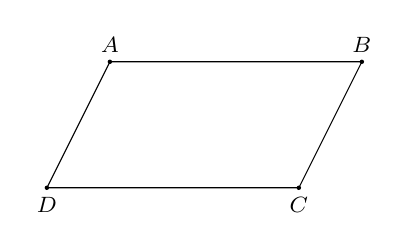
\begin{tikzpicture}[scale=0.8,font=\footnotesize,>=stealth]
			\coordinate[label=above:$A$] (A) at (0,2);
			\coordinate[label=above:$B$] (B) at (4,2);
			\coordinate[label=below:$C$] (C) at (3,0);
			\coordinate[label=below:$D$] (D) at (-1,0);
			\draw (A)--(B)--(C)--(D)--(A); 
			\foreach \diem in {A,B,C,D}\fill (\diem)circle(1pt);
			\end{tikzpicture}
		\end{center}
		Ta có $\vec{AB}=(-1;-4)$ và $\vec{BC}=(2;2)$. \\
		Suy ra $\vec{AB}$ và $\vec{BC}$ không cùng phương.\\
		Gọi $D(x;y)$.\\
		Tứ giác $ABCD$ là hình bình hành khi và chỉ khi 
		\begin{center}
			$\vec{AD}=\vec{BC} \Leftrightarrow (x-2;y-5)=(2;2) \Leftrightarrow  \heva{&x-2=2\\&y-5=2}
			\Leftrightarrow
			\heva{&x=4\\&y=7.} $
		\end{center}
		Vậy $D(4;7)$.
	}
\end{bt}
